%% LyX 2.1.4 created this file.  For more info, see http://www.lyx.org/.
%% Do not edit unless you really know what you are doing.
\documentclass[english,msc,oneside]{ubcthesis}
\usepackage{mathptmx}
\usepackage{helvet}
\renewcommand{\ttdefault}{cmtt}
\renewcommand{\familydefault}{\rmdefault}
\usepackage[T1]{fontenc}
\usepackage[latin9]{inputenc}
\usepackage{geometry}
\geometry{verbose,lmargin=3.5cm,rmargin=3.5cm}
\usepackage{color}
\usepackage{babel}
\usepackage{prettyref}

\usepackage{float}
\usepackage{url}
\usepackage{amsmath}
\usepackage{amsthm}
\usepackage{amssymb}
\usepackage{graphicx}
\usepackage{esint}
\usepackage[numbers]{natbib}

\usepackage[unicode=true,pdfusetitle,
 bookmarks=true,bookmarksnumbered=false,bookmarksopen=false,
 breaklinks=false,pdfborder={0 0 1},backref=section,colorlinks=true]
 {hyperref}
\usepackage{cleveref}
\makeatletter

%%%%%%%%%%%%%%%%%%%%%%%%%%%%%% LyX specific LaTeX commands.

\let\pr@chap=\pr@cha
%% A simple dot to overcome graphicx limitations
\newcommand{\lyxdot}{.}


%%%%%%%%%%%%%%%%%%%%%%%%%%%%%% Textclass specific LaTeX commands.
\usepackage{enumitem}		% customizable list environments
\newlength{\lyxlabelwidth}      % auxiliary length 

%%%%%%%%%%%%%%%%%%%%%%%%%%%%%% User specified LaTeX commands.

\usepackage{afterpage}

\usepackage{float}

%\usepackage{alltt}

\usepackage{longtable}

\usepackage{graphicx}

\usepackage{lscape}

%\usepackage[numbers,sort&compress]{natbib}

\usepackage{psfrag}
\usepackage{multicol}

%\usepackage[hypertex,final=true,unicode=true, pdfusetitle,bookmarks=true,bookmarksnumbered=false,bookmarksopen=true,breaklinks=true,pdfborder={0 0 1},backref=true,colorlinks=true,citecolor=black, filecolor=black, linkcolor=black, urlcolor=black]{hyperref}
\usepackage{hyperref}
\usepackage{caption}
\captionsetup[figure]{font=small}

\hypersetup{
hypertex=true,
unicode=true, pdfusetitle,
bookmarks=true,
bookmarksnumbered=false,
bookmarksopen=true,
breaklinks=true,
pdfborder={0 0 1},
backref=true,
colorlinks=true,
citecolor=black,
filecolor=black,
linkcolor=black,
urlcolor=black
}

% These commands are optional.  The defaults are shown.  You only
% need to include them if you need a different value
\institution{Universidade de S\~ao Paulo}

% If you are at the Okanagan campus, then you should specify these
% instead.
%\faculty{The College of Graduate Studies}
%\institutionaddress{Okanagan}
\faculty{Instituto de F\'isica}
\institutionaddress{ R. do Mat\~ao, 1371 - Butant\~a, S\~ao Paulo}

% You can issue as many of these as you have...
%\previousdegree{B.Sc., The University of British Columbia, 1999}
%\previousdegree{M.Sc., The University of British Columbia, 2001}
%\previousdegree{Ph.D., Massachusetts Institute of Technology, 2005}

% You can override the option setting here.
% \degreetitle{Jack of All Trades}

% These commands are required.
\title{Indirect exchange and Kondo interactions in Majorana-double quantum dot systems.}
%\subtitle{Master Thesis}
\author{Jes\'us David Cifuentes Pardo}
\copyrightyear{2017}
\submitdate{\today}

\program{Condensed Matter Physics}

% These commands are presently not required for UBC theses as the
% advisor's name and title are not presently required anywhere.
%\advisor{Ariel R.~Zhitnitsky}
%\advisortitle{Professor of Physics}

% One might want to override the format of the section and chapter
% numbers.  This shows you how to do it.  Note that the current
% format is acceptable for submission to the FoGS: If you wish to modify
% these, you should check with the FoGS explicity. prior to making
% the modifications.
\renewcommand\thepart         {\Roman{part}}
\renewcommand\thechapter      {\arabic{chapter}}
\renewcommand\thesection      {\thechapter.\arabic{section}}
\renewcommand\thesubsection   {\thesection.\arabic{subsection}}
\renewcommand\thesubsubsection{\thesubsection.\arabic{subsubsection}}
\renewcommand\theparagraph    {\thesubsubsection.\arabic{paragraph}}
\renewcommand\thesubparagraph {\theparagraph.\arabic{subparagraph}}

% Following now set in LyX
%\setcounter{tocdepth}{2}
%\setcounter{secnumdepth}{2}

% Here is an example of a "Program" environment defined with the
% "float" package.  The list of programs will be stored in the file
% ubcsample.lop and the numbering will start with the chapter
% number.  The style will be "ruled".
\floatstyle{ruled}
\newfloat{Program}{htbp}{lop}[chapter]
\AtBeginDocument{%
\let\ref\autoref
\renewcommand\equationautorefname{\@gobble}
}

\@ifundefined{showcaptionsetup}{}{%
 \PassOptionsToPackage{caption=false}{subfig}}
\usepackage{subfig}
\makeatother



\newcommand{\nhat}{\hat{n}}
\newcommand{\veck}{\textbf{k}}
\newcommand\ep{\epsilon}
\newcommand\g{\gamma}
\newcommand\s{\sigma}
\newcommand\up{\uparrow}
\newcommand\dw{\downarrow}
\newcommand\down{\downarrow}
\newcommand{\ed}[1]{\ep_{d#1}}
\newcommand{\ket}[1]{\vert #1 \rangle}
\newcommand{\ann}{a^{\dagger}}
\newcommand{\dann}{d^{\dagger}}
\newcommand{\gammaA}[1]{\gamma_{A,#1}}
\newcommand{\gammaB}[1]{\gamma_{B,#1}}
%\newcommand{\bra}[3]{\langle {#3} \vert}

\newcommand{\super}{\vert \Delta \vert}

\begin{document}
\mainmatter
\maketitle
\begin{abstract}
The interesting prospect of creating devices that could realize quantum
computation operations by exploring the non-Abelian character of Majorana
quasiparticles has spurred the so-called \textquotedblleft search
for Majorana fermions\textquotedblright{} in condensed matter systems
\citep{kitaev_unpaired_2001}. As recently as 2012, experimental works
reporting the detection of such quasiparticles have been put forward
\citep{alicea_majorana_2010,alicea_new_2012}. Later works \citep{liu_detecting_2011,lee_kondo_2013,vernek_subtle_2014,deng_majorana_2016},
including a recent paper published by the advisor of this dissertation
and collaborators \citep{ruiz-tijerina_interaction_2015}, set out
to explore the interplay of such Majorana zero-modes with strongly
interacting systems such as semiconductor quantum dots, which can
be readily integrated in the device. This research project aims to
expand these interesting connections by studying a double quantum
dot coupled to metallic leads and to a topological superconductor
supporting edge Majorana zero modes. The interplay of Kondo correlations
(between each dot and the leads), exchange interaction (between the
dots) and Kondo-Majorana interaction (between the dot and the Majorana
modes) will be investigated. The work involves the numerical calculation
of the many-body spectrum of the system with Wilson\textquoteright s
Numerical Renormalization Group (NRG) technique.
\begin{description}
\item [{}]~{\small \par}
\end{description}
\end{abstract}




%\tableofcontents{}
\chapter{Motivation}

In 2001 Alexei Yu. Kitaev presented a model for implementing qubits
that could face the problem of high decoherency in quantum computation \citep{kitaev_unpaired_2001}. Kitaev's idea was centered in using the properties of an exotic quasi-particle that appears at the edges of a quantum superconducting chain. This quasi-particle receives the name of Majorana Fermion, is characterized for being its own anti-particle, thus it has no charge or spin. It also presents non-Abelian statistics, a desired property to implement fault-tolerant quantum computers\citep{kitaev_fault-tolerant_2003}. These majorana fermions where theoretically predicted since the 1930's by one of the genius of the era, Ettore Majorana \citep{wilczek_majorana_2009}.
Although no fundamental Majorana-particle has been discovered to the
date, Kitaev's model inspired the pursue of majorana fermions as
quasi-particles in a novel exotic class of materials known as topological
superconductors (TS)\citep{fu_superconducting_2008,sato_non-abelian_2009,alicea_new_2012}.
\\

The last five years have been full of excitement, as new experiments
have turned some of the theoretical predictions of the 1990s and 2000s
into a reality. Very recently the first evidence of Majorana end states
in TS has been found in multiple experiments \citep{mourik_signatures_2012,das_zero-bias_2012,deng_anomalous_2012}
following the prescription by \citet{oreg_helical_2010} and \citet{lutchyn_majorana_2010}.
These experiments have been based on tunneling spectroscopy in junctions
between TS and non metallic (NM) leads, where resonances have been
observed at zero energy, consistent with the presence of Majorana
zero\textendash energy modes.\\

A downside of the tunneling spectroscopy technique in this case, is
that it probes not only the end of the Topological Superconductor(TS), but its bulk as well ,
which completely destroys the qubit information. A less destroying
model presented by \citet{liu_detecting_2011} consists consists in attaching a Quantum Dot (QD) to the edges of a majorana chain in the topological phase and executing transport measurements through the QD \cite{liu_detecting_2011} . The majorana mode at the end of the chain then leaks inside the QD \cite{vernek_subtle_2014} which produces a zero-bias conductance peak of half a quanta $\frac{e^{2}}{2h}$ through the dot. This is a majorana signature which produces half of the expected peak by a regular fermion.\\

In fact, this phenomenon is similar to the $\frac{e^{2}}{h}$ conductance peak caused by the Kondo effect \citep{hewson_kondo_1997}. Since topological superconductors and the Kondo effect could coexist at temperatures of a few mili-kelvins, it should be possible to observe combined Kondo-Majorana physics in this type of devices. This idea motivated an NRG study of a Quantum dot-Majorana hibrid system in the Kondo regime  \citep{ruiz-tijerina_interaction_2015}. \\

\begin{figure}[t]
    \centering
    \includegraphics[scale=0.4]{IMAGES/Kondo-MajoranaCond.png}
    \caption{\label{Fig-Kondo-Majorana conductance}(a) QD spin-down
    density of states. Because this channel couples to the Majorana mode,
    it displays the characteristic zero-bias signature of amplitude
    $\frac{e^{2}}{2h}$. (b) QD spin-up density of states,
    displaying the zero-bias peak of the Kondo effect, with
    unit amplitude. (c) Zero-bias conductance of the QD coupled
    to the Majorana mode, as a function of the QD energy level ($\lambda$
    parameterizes the strength of the Majorana-QD tunnel coupling).
    The presence of the spin-up Kondo resonance enhances the
    QD conductance in particle-hole symmetry ($V_{g}=0$),
    but quickly disappears as the QD level is detuned from this point.
    The spin-down Majorana signature, on the other hand, is
    robust {[}7{]}, leaving a residual conductance of $\frac{e^{2}}{2h}$.
    \protect\Source{\citep{ruiz-tijerina_interaction_2015}}.}
\end{figure}

This study revealed that transport measurements
through the quantum dot will show contributions to the enhanced conductance
coming from the Kondo effect and the Majorana mode: The Majorana mode
at the end of the wire will migrate into one of the quantum dot spin channels,
giving rise to a zero\textendash energy peak in the density of states
(\ref{Fig-Kondo-Majorana conductance}a)) contributing a conductance
of $\frac{e^{2}}{2h}$(\ref{Fig-Kondo-Majorana conductance}c)). The
zero\textendash bias peak from the Kondo effect appears in the other
spin channel (\ref{Fig-Kondo-Majorana conductance}b)), contributing
a conductance of $\frac{e^{2}}{h}$. Then, the Kondo effect can be
\textquotedblleft turned off\textquotedblright{} through gate voltages
and magnetic fields, leaving only the Majorana contribution. Clear
evidence of the destruction of the Kondo peak will appear in the conductance,
allowing for a distinction between Majorana and Kondo signatures.\\



 Apart from not destroying the entire qubit-information the QD-method has another insight.  This is the possibility of manipulating  Majorana fermions  in multidot systems by shifting the QD gate voltages and tunnel couplings which brings possible applications in  braiding procedures. The simplest system where Majorana manipulation is possible is  a  Double Quantum Dot (DQD) coupled to a majorana chain. By tuning the QD gate voltages and the majorana coupling we will be able to probe the mobility of the majorana modes through the dots. \\
 
In addition, when both dots are coupled to the lead the Double Quantum Dot exhibits an anti-ferromagnetic interaction known as  Ruderman-Kittel-Kasuya-Yosida (RKKY) \cite{ruderman_indirect_1954,kasuya_theory_1956,yosida_magnetic_1957}. On the other hand, when only one dot is coupled  and the second Dot is indirectly attached through the first dot,  the Kondo effect is annihilated due to the destructive interference  generated by extra dot \cite{dias_da_silva_transmission_2008}. Both cases reveal interesting results for majorana manipulation and hybrid Kondo-Majorana systems.


\section{Structure}

This thesis is integrated by $4$-major chapters . In  \ref{chap:Preliminaries}, we will take a review to the basis of quantum transport in single electron transistors, the Anderson model and the emergence of the Kondo effect in quantum dots. 

In \ref{chap: Methods} contains a description of the methods that we will use to study the Double Quantum Dot-majorana system. The  methods  are the Zubarev's ballistic transport\cite{zubarev_double-time_1960} for non-interacting systems and Wilson's Numerical Renormalization
Group (NRG) technique \citep{wilson_renormalization_1975} for interacting systems. We will use the Double Quantum Dot case as major example to explain both methods. Hence the background information about double quantum dots systems will be presented in this chapter. 

The \ref{chap:Majorana} changes the subject, leading us to the mean topic of this thesis, Majorana fermions. The discussion will start with the Kitaev chain addressing its main characteristics such as topological characterization and non-abelian statistics . Then we take a look to the real implementations of majorana chains were we will discuss the most recent experimental accomplishments  in the area.  At the end, we face the the problem of a hybrid Quantum Dot-Majorana system using the methods described in \ref{chap: Methods}.

Using the methods from \ref{chap: Methods} and the previous acquired experience with the Double Quantum Dot and the Quantum Dot-Majorana , we address in \ref{chap:Results} the  Double Quantum Dot-Majorana system. We will study several procedures  mainly focused in the manipulation of majorana fermions and the combined effects of Kondo-Majorana physics. 








\chapter{Preliminaries \label{chap:Preliminaries}}



In this preliminary chapter we will give a brief description description about transport processes in quantum dots (QDs). We will discuss basic aspects about single electron transistors, the application of the Anderson impurity model in QDs and the subsequent emergence of the Kondo effect, one of the main condensed matter problems of the $20^{th}$-century. 

%-------------------------------------------------------------
%Here goes the introduction of transport between quantum dots. stil need to add important considerations like the smooth varying DOS. Not so discrete. 
%Assumption: 
%   1-Only the level immediately at the bottom of the fermi       level is considered
\section{Transport process in quantum dots (QDs) \label{sec:trans}}
% --------------Figure-------------------------
\begin{figure}[hbt]
    \centering
    \subfloat[\label{QD-figuresA}\label{QD-figures}]{\includegraphics[scale=0.3]{IMAGES/Preliminars/VerticalQD.png}}\hspace{6mm}
    \subfloat[\label{QD-figuresB}]{\includegraphics[scale=0.4]{IMAGES/Preliminars/QD-horizontal.png}}
    \caption{ \label{fig:QD} a) Vertical quantum dot.  b)Atomic force microscopy
    picture of two coupled lateral QDs (bright central circles). Gates 1 and 2 act as drain and source voltage. A negative
    voltage is applied at gates $A$,$B$ to allow the formation of the droplets inside the free space in the 2D electron gas. \protect\Source{Adapted from \cite{holleitner_probing_2002}} }
\end{figure}

Quantum mechanical effects are visible when the system size is of the order of the de Broglie wavelength \citep[(1.1)]{bimberg_quantum_1999}
\[
\lambda_{f}=\frac{h}{\sqrt{3m_{\mathsf{eff}}k_{B}T}}
\]
 where $m_{\mathsf{eff}}$ is the electron effective mass in the crystal. Since $m_{\mathsf{eff}}$ can be much smaller than the free electron mass in some semiconducting materials, size quantization effects can be observed at system of sizes $\sim100\mbox{nm}$ \cite{sindel_numerical_2005}. A $0$D quantum system is a device confined in the three spacial dimensions up to this length-scale. This type of device receive the name of quantum dot (QD). 

\begin{figure}[tb]
    \centering
    \includegraphics[scale=0.5]{IMAGES/Preliminars/specDot.png}
    \caption{Representation of the Density of States of a QD. The gate potential $V_G$ can be tuned to change the Fermi energy of the dot. 
    \label{fig:specDots}}
\end{figure}


\begin{figure}[t]
     \centering
    
     \subfloat[ \label{fig:QD-transport}]{\includegraphics[scale=0.7]{IMAGES/Preliminars/QD-Transport.png}}
    \subfloat[\label{fig:QD-Blockade}]{\includegraphics[scale=0.3]{IMAGES/Preliminars/QD-Blockade1.png}}
     \caption{ \label{fig:QD-Trans} (a) Representation of transport through QD. The red curve represents the hybridized energy level. The gate voltage tunes this level. In the case represented, the energy level is in the middle of the drain and source voltages allowing transport between the leads. (b) Charging diagram of a quantum dot. Differential conductance dependence over the gate voltage $V_G$ and the source-drain voltage $(V_{SD}=V_{S}-V_{D} )$. Coulomb blockade occurs at the diamond-shaped regions with zero conductance. At these regions the number of electrons is constant and increases $1$ by $1$ when the gate voltage is scaled up.  \protect\Source{(b) Adapted from \cite{sindel_numerical_2005}  }}
\end{figure}

  Nowadays, QDs can be manufactured in different substracts, geometries and  and orientations \citep{bimberg_quantum_1999}. They can be integrated in structures like double quantum dots (\ref{fig:QD}(a)) or can even be grown vertical to the based 2D-electron gas (\ref{fig:QD}(b)). The precise experimental control over these devices allows to design atom-like structures with tunable energy levels. This has important applications on laser physics and in the implementation of single electron transistors. 
  % According to their orientation with respect to the based 2D-plane  two main types of QDs can be distinguished : Vertical (Figure \ref{QD-figuresA}) and lateral (Figure \ref{QD-figuresB}) QDs. 


  

   Ideally, the energy spectrum of a QD is a discrete set of energy levels resembling the spectrum of an atom. This atom-like structure is usually connected to three main gates (See \ref{fig:QD-Trans}(a)). Two of them are the source and the drain with voltages $V_S$ and $V_D$, used to control the electric gradient through the QD. When the QD is connected to these leads these energy levels are hybridized with respect to a broadening parameter $\Gamma$ which increases as the square of the source-drain voltage $V_{SD}$ 
\begin{equation}
    \Gamma \propto \pi \Vert V_{SD} \Vert^2
\end{equation}
\noindent This broadening is depicted in \ref{fig:specDots}. Ideally, $\Gamma \ll \Delta E$ is smaller enough such that the energy levels do not overlap each other. 

The third gate is the gate voltage $V_G$ which allows to tune the energy levels of the dot with high  precision. With this three gates it is possible to execute transport measurements through a QD . An electron can pass from the source to the drain if there is an energy level in the middle of the two voltages, just as in \ref{fig:QD-Trans}(a). If this condition is not satisfied,  the dot enters into a Coulomb blockade region without  electron transport between both leads as can be observed in \ref{fig:QD-Trans}(b)). Inside the Coulomb blockade regions (black diamonds) the number of electrons is constant. When increasing $V_G$ a single electron enters into the dot each time the system makes a transition between blockade regions. Since all of these effects can be controlled precisely with the gate voltage, the system described is indeed a single electron transistor (SET).  

Note that when $V_{SD}=0$, the condition for conductance can still be satisfied if there is an hybridized state at the level of $V_S = V_D$,  the Fermi energy. This situation receives the name of zero-bias conductance peak (ZBCP). The effects that can cause robust ZBCPs are quite interesting. In this thesis were will study two of them. The Kondo effect and the Majorana zero modes. 






% Indeed we can model an ideal single-electron QD as a quantum well
% with a negative constant potential inside the dot . For example an
% spherical quantum dot with radius $R$ will take the following Schr�dinger
% Hamiltonian 

% \[
% H\Psi(r)=\left(\frac{\hbar^{2}}{2m^{*}}\nabla^{2}+V(r)\right)\Psi(r)\ ,\ \textrm{with }V(r)=\begin{cases}
% -V_{0} & r<R\\
% 0 & r\geq R
% \end{cases}.
% \]


% The 
% the energy level spacing is  \citep[Equation (5.44)]{bimberg_quantum_1999}

% \[
% \delta E\propto\frac{1}{R^{2}}.
% \]



%------------------------------------------------------------
\section{The Anderson Model \label{sec:Anderson}}
% The key ingredient in the Kondo phenomena is the presence of magnetic impurities whose states are hybridized to conduction electron in the metal. To study this idea the physics Nobel prize winner Philip Anderson created a model that simulated the quantum interaction between the impurity and the conduction band \citep{anderson_localized_1961}. The Anderson Model can be applied to different problems. In this thesis we are mainly interested in the study of artificially manufacture impurities better known as quantum dots.   

 %Here the study of the  magnetic impurities in metals responsible for the Kondo effect, as well as artificial impurities like quantum dots. 
 The Anderson model is used to describe quantum impurity systems \citep{anderson_localized_1961}. A quantum dot attached to a metallic lead is basically an artificial impurity that can be experimentally designed, modified and manipulated. Hence QDs are the perfect type of structure to test the Anderson mode.   

 Due to the small confinement space inside these dots,  Coulomb repulsion is relevant. However, it is usually impossible to provide a complete analytical description of these kind of systems due to the high correlations generated by this factor. Instead, we can obtain an overall description of the transport through the impurity by neglecting this Coulomb repulsion. This will allow us to obtain some analytic intuition of the models  before adventuring with long-lasting numerical simulations of interacting models. During this thesis, we will consider these two regimes as follows
\begin{itemize}
    \item \textbf{Non-interacting systems:} Coulomb repulsion is not relevant . In this case, spin-$\uparrow$ and spin-$\dw$ channels are independent. They can be solved analytically through the equations of motion (\ref{sec:transport}). 

    \item \textbf{Interacting systems:} The Coulomb repulsion is relevant. The repulsion factor will be defined by the factor $U$ which will take a fix value during the entire project. In this case, spin-$\uparrow$ and spin-$\dw$ channels are not independent since the Coulomb repulsion limits the number of particles inside each dot. We will use the Numerical Renormalization Group to treat this case. The intuition acquired from non-interacting systems will help us to select the input parameters of the algorithm.  
\end{itemize}


%The Anderson model takes in account both regimes and  the only difference in each case will be the value of $U$ parameter ($U=0$ non-interacting , $U>0$ interacting). 

To begin the description of the Anderson model, first consider that we have a QD (impurity) coupled to the conduction band of a metallic lead. We will define a Coulomb repulsion factor $U_i$, which will be set to $0$ if the system is non-interacting . Using the Hund rules, we know that the energy levels inside the dot should be filled from lower to higher energies with two electrons with different spin at each state. Each pair of electrons will interact magnetically and electrically. In addition, there is and energy term associated to each electron and a Zeeman splitting factor in case a $\hat{z}$-directed magnetic field $B$ is placed.  Considering these interactions, we can obtain a very general expression in second quantization for the QD Hamiltonian
of the form \citep[(3.2)]{sindel_numerical_2005}

\begin{equation}
H_{d}=\sum_{i\sigma}\epsilon_{i}d_{i\sigma}^{\dagger}d_{i\sigma}+\sum_{i}U_{i}\hat{n}_{i\uparrow}\hat{n}_{i\downarrow}+\sum_{\sigma\sigma',i\neq j}U_{ij}\hat{n}_{i\sigma}\hat{n}_{j\sigma'}-\mu_{B}gB\sum_{i}S_{i}^{z}+J\sum_{i\neq j}\mathbf{S}_{i}\cdot\mathbf{S}_{j},
\end{equation}




\noindent where $\sigma\in\{\uparrow,\downarrow\}$, $d_{i\sigma}^{\dagger}\left(d_{i\sigma}\right)$
is the dot creation(annihilation) operator,$\hat{n}_{i\sigma}:=d_{i\sigma}^{\dagger}d_{i\sigma}$
is the particle number, $\mathbf{S}_{i}$ is the spin-vector, $\epsilon_{i}$
is the energy of the $i^{\mbox{th}}$-level in the dot, $U_{i}$ is
the Coulomb repulsion between electrons in the same energy level $i$,
$U_{ij}$ is the Coulomb interaction between electrons in different
levels (And therefore smaller than $U_{i}$), \textbf{$B$} is an
applied magnetic field in the $\hat{z}$-direction causing a Zeeman splitting and $J$ is the
term representing the spin coupling between distinct levels

At low temperatures, the quantum interactions occur only with the closest energy level to the Fermi energy. Hence, we can make a single-level approximation, neglecting the other energy levels. Hence, we can set the parameters $U_i=U_{ij}=0$ and $J=0$ , which significantly reduces the complexity of the dot Hamiltonian \\


\begin{equation}
    H_{d}=\sum_{\sigma}\epsilon_{}d_{\sigma}^{\dagger}d_{\sigma}+U\hat{n}_{\uparrow}\hat{n}_{\downarrow}-\mu_{B}gBS^{z}. \label{eq:hdot}
\end{equation}

Besides to the dot Hamiltonian, we need to consider the energy of the electrons in the lead $H_{lead}$ and the dot-lead interaction $H_{int}$. We can model  the conduction band of the lead as an electron gas with the following Bloch Hamiltonian
\begin{equation}
H_{lead}  =  \sum_{\mathbf{k}\sigma l}\epsilon_{\mathbf{k}l}c_{\mathbf{k}\sigma l}^{\dagger}c_{\mathbf{k}\sigma l}. 
\end{equation}

\noindent where $\mathbf{k}$ represents the possible crystal momentums in the
leads, $l\in\{S,D\}$, $c_{\mathbf{k}\sigma l}^{\dagger}(c_{\mathbf{k}\sigma l})$
creates(annihilates) an electron with momentum $\mathbf{k}$ and spin
$\sigma$ in the lead $l$, $\epsilon_{\mathbf{k}l}$ is the energy
of the electron in the leads. 

On the other hand, the interaction between the dot and the leads is then given by 
\begin{equation}
H_{int} = \sum_{\mathbf{k}\sigma l}V_{\mathbf{k}l}c_{\mathbf{k}\sigma l}^{\dagger}d_{\sigma}+V_{\mathbf{k}l}^{*}d_{\sigma}^{\dagger}c_{\mathbf{k}\sigma l},
\end{equation}
%\begin{eqnarray*}
%H_{lead} & = & \sum_{\mathbf{k}\sigma l}\epsilon_{\mathbf{k}l}c_{\mathbf{k}\sigma l}^{\dagger}c_{\mathbf{k}\sigma l}\\

%\end{eqnarray*}

\noindent where $V_{\mathbf{k}l}$ is a hopping exchange
term between the leads and the QD. 


The sum of these three interactions receives the name of Anderson Model. 
\begin{eqnarray}
H & = & H_{d}+H_{lead}+H_{int}\nonumber \\
 & = & \sum_{\sigma}\epsilon_{}d_{\sigma}^{\dagger}d_{\sigma}+U\hat{n}_{\uparrow}\hat{n}_{\downarrow}-\mu_{B}gBS^{z}+\sum_{\mathbf{k}\sigma l}\epsilon_{\mathbf{k}l}c_{\mathbf{k}\sigma l}^{\dagger}c_{\mathbf{k}\sigma l}+\sum_{\mathbf{k}\sigma l}V_{\mathbf{k}l}c_{k\sigma l}^{\dagger}d_{\sigma}+V_{\mathbf{k}l}^{*}d_{\sigma}^{\dagger}c_{\mathbf{k}\sigma l}.\label{eq:Anderson}
\end{eqnarray}

In this project, we will make two extra modifications to this system. Using the anti-commutation properties of the fermion operators

% \begin{equation}
% H=H_{d}+H_{lead}+H_{int}=\sum_{\sigma}\epsilon_{}d_{\sigma}^{\dagger}d_{\sigma}+U\hat{n}_{\uparrow}\hat{n}_{\downarrow}+\sum_{\mathbf{k}\sigma l}\epsilon_{\mathbf{k}l}c_{\mathbf{k}\sigma l}^{\dagger}c_{\mathbf{k}\sigma l}+V_{\mathbf{k}l}c_{\mathbf{k}\sigma l}^{\dagger}d_{\sigma}+V_{\mathbf{k}l}^{*}d_{\sigma}^{\dagger}c_{\mathbf{k}\sigma l}.\label{eq:hamB0}
% \end{equation}
\[
\left\{ d_{\sigma}^{\dagger},d_{\sigma'}\right\} =\delta_{\sigma\sigma'}\ ,\ \left\{ d_{\sigma}^{\dagger},d_{\sigma'}^{\dagger}\right\} =\left\{ d_{\sigma},d_{\sigma'}\right\} =0,
\]
\noindent we get


\begin{eqnarray*}
\left(d_{\up}^{\dagger}d_{\up}+d_{\down}^{\dagger}d_{\down}-1\right){}^{2} & = & \sum_{\sigma}\left(d_{\sigma}^{\dagger}d_{\sigma}\right)^{2}-2\sum_{\sigma}d_{\sigma}^{\dagger}d_{\sigma}+2d_{\up}^{\dagger}d_{\up}d_{\down}^{\dagger}d_{\down}-1\\
 & = & 2d_{\up}^{\dagger}d_{\up}d_{\down}^{\dagger}d_{\down}-\sum_{\sigma}d_{\sigma}^{\dagger}d_{\sigma}-1.
\end{eqnarray*}

\noindent And replacing this in \eqref{eq:hdot} we obtain a  nice spin-symmetric form of the dot Hamiltonian

\begin{equation}
    \left(\epsilon_{}+\frac{U}{2}\right)d_{\sigma}^{\dagger}d_{\sigma}+\frac{U}{2}(d_{\sigma}^{\dagger}d_{\sigma}-1)^{2}-\mu_{B}gBS^{z}. 
    \label{eq:hdot2}
\end{equation}

In addition, it is possible to do a linear transform to the lead operators 
\begin{equation}
    \frac{1}{\sqrt{V_{S}^{2}+V_{R}^{2}}}\left[\begin{array}{cc}
V_{S} & V_{R}\\
-V_{R} & V_{S}
\end{array}\right]\left[\begin{array}{c}
c_{\mathbf{k}\sigma S}\\
c_{\mathbf{k}\sigma D}
\end{array}\right]=\left[\begin{array}{c}
c_{\mathbf{k}\sigma+}\\
c_{\mathbf{k}\sigma-}
\end{array}\right].
\end{equation}
\noindent After this transformation the operator will be decoupled from the dot Hamiltonian $c_{\mathbf{k}\sigma-}$ . This implies that we can suppose that the  dot is coupled with just one lead. In the following chapters we will maintain this convention. 


%------------------------------------------------------------
\section{The Kondo Effect \label{sec:Kondo} }


\begin{figure}[t]
     \centering
    
     \subfloat[ \label{fig:KondoTemp}]{\includegraphics[scale=0.6]{IMAGES/Preliminars/KondoTemp.png}}
    \subfloat[\label{fig:KondoKloud}]{\includegraphics[scale=1.3]{IMAGES/Preliminars/kondoCloud.png}}
     \caption{ \label{fig:Kondo} (a) Resistivity minimum near the Kondo temperature $T_k$. (b) Kondo cloud formed by a singlet grouped around the impurity divided in spin-$\up$,spin-$\dw$ regions.   \protect\Source{ Adapted from a) \cite{Kondo_deBoer1934} , b) \cite{Ternes_2008}  }}
\end{figure}


The Kondo effect is still regarded as one of the biggest condensed matter problems in the 20th century. There was an uncountable number of experimental and theoretical physicist that contributed to this problem . The most renown are probably the physicists Jacques Friedel, Jun Kondo and the two Nobel prizes Philip Anderson and Kenneth Wilson \citep{hewson_kondo_1997}. 

The history of the Kondo effect began in the early 1930s. By that time it was known that the resistivity of a metal is regulated by different scattering interactions against lattice phonon vibrations $\rho_{phonon} \sim T^5$, other electrons $\sim T^2$ and static impurities, which is temperature independent. The form of these contribution clearly implies that the resistivity should decay uniformly with a decreasing temperature. Nevertheless, some groundbreaking experiments revealed the observation of a resistance minimum in some metals at temperatures lower than $10K$ \cite{Kondo_deBoer1934}(See \ref{fig:Kondo} (a)). 

This phenomenon intrigued the scientific community for the following decades until the year 1964 when the physicist  Jun Kondo gave the first convincing solution to this puzzle. Kondo attributed the phenomenon to the scattering of the electrons due to the spin-interaction with a small concentration of magnetic impurities in the metal. To describe it he proposed the following interaction Hamiltonian

\begin{align}
H_K &= 2J\hat{\textbf{S}}\cdot \hat{\textbf{s}} \\
&=  J (2S_z s_z + S_+s_- +S_-s_+),
\end{align}
with $S_\pm = S_x \pm iS_y$. The Hamiltonian $H_K$ which is better known as the Kondo s-d model describes the spin interaction between the spin of the impurity $\hat{\textbf{S}}$ and the spin of the particles in the metal $\hat{\textbf{s}}$.

Kondo took $H_K$ as a perturbation of the electron gas in the metallic lead, with $J$ the perturbation parameter. While the first order led to no important contribution, Kondo was able to obtain on second order perturbation theory a logarithmic correction on the temperature in the resistivity of the form 

\begin{equation}
\rho_{imp} \propto \ln{\frac {
T_K }{T}},
\end{equation}
where $T_K$ received the name of Kondo temperature. Summing up this term to the other resistivity contributions we obtain the full expression 
\begin{equation}
{\displaystyle \rho_{metal} (T)=\rho_{imp}+a_{e}T^{2}+b_{Phonon}T^{5} + c_{m}\ln {\frac {
T_K }{T}}}.
\label{logKondo}
\end{equation}
\noindent When $T< T_K$ the term $ \ln {\frac {
T_K }{T}}$ increases. Eventually, it compensate the decaying resistivity which finally explained the  resistance minimum. 

Although Kondo's explanation was initially very successful it also presented a troublesome outcome. The logarithmic term introduced by Kondo diverges when the temperature approximates to $0$, hence proving to be inefficient at temperatures well bellow $T_K$. Going to the following orders in perturbation theory also led to divergent contributions to the  resistivity. This led physicists  to explore non-perturbative approaches to solve the Kondo effect. 

By that time, Anderson had already created his famous impurity model. One of his main contributions was the inclusion of the Hubbard term to represent the Coulomb interaction inside the dot, which proofed to be fundamental to understand the Kondo effect.Nonetheless, the Anderson model was a huge numerical challenge. The problem was finally solved by Kenneth Wilson, who was able to effectively diagonalize the Anderson model using a numerical method that combines ideas from scalability and the renormalization group. 

Wilson's explanation solved the Kondo problem almost completely. It turned out that bellow the Kondo temperature \cite{sindel_numerical_2005}, which is around
\begin{equation}
k_BT_K = \frac{1}{2}\sqrt{U\Gamma}e^{\epsilon(\epsilon+U)/\Gamma U} ,
\end{equation}

\noindent the impurity entangles with the low-energy electrons forming a strongly correlated many-body singlet. This singlet surrounds the impurity in an structure formed by alternating regions of spin-$\up$ and spin-$\dw$ particles called the Kondo cloud (See \ref{fig:Kondo}(b)). The Kondo cloud was the first evidence of an entangled many body state, and is predicted to have an astonishing correlation length between $0.1\mu m$ to $10 \mu m$. This is a huge number if we think that the impurity(or QD) can have a radius bellow $1nm$. Finally, the minimum in the resistivity is produced when the conduction electrons scatter with the Kondo cloud. 

\subsection{Kondo Effect in QDs}

\begin{figure}
  \centering
  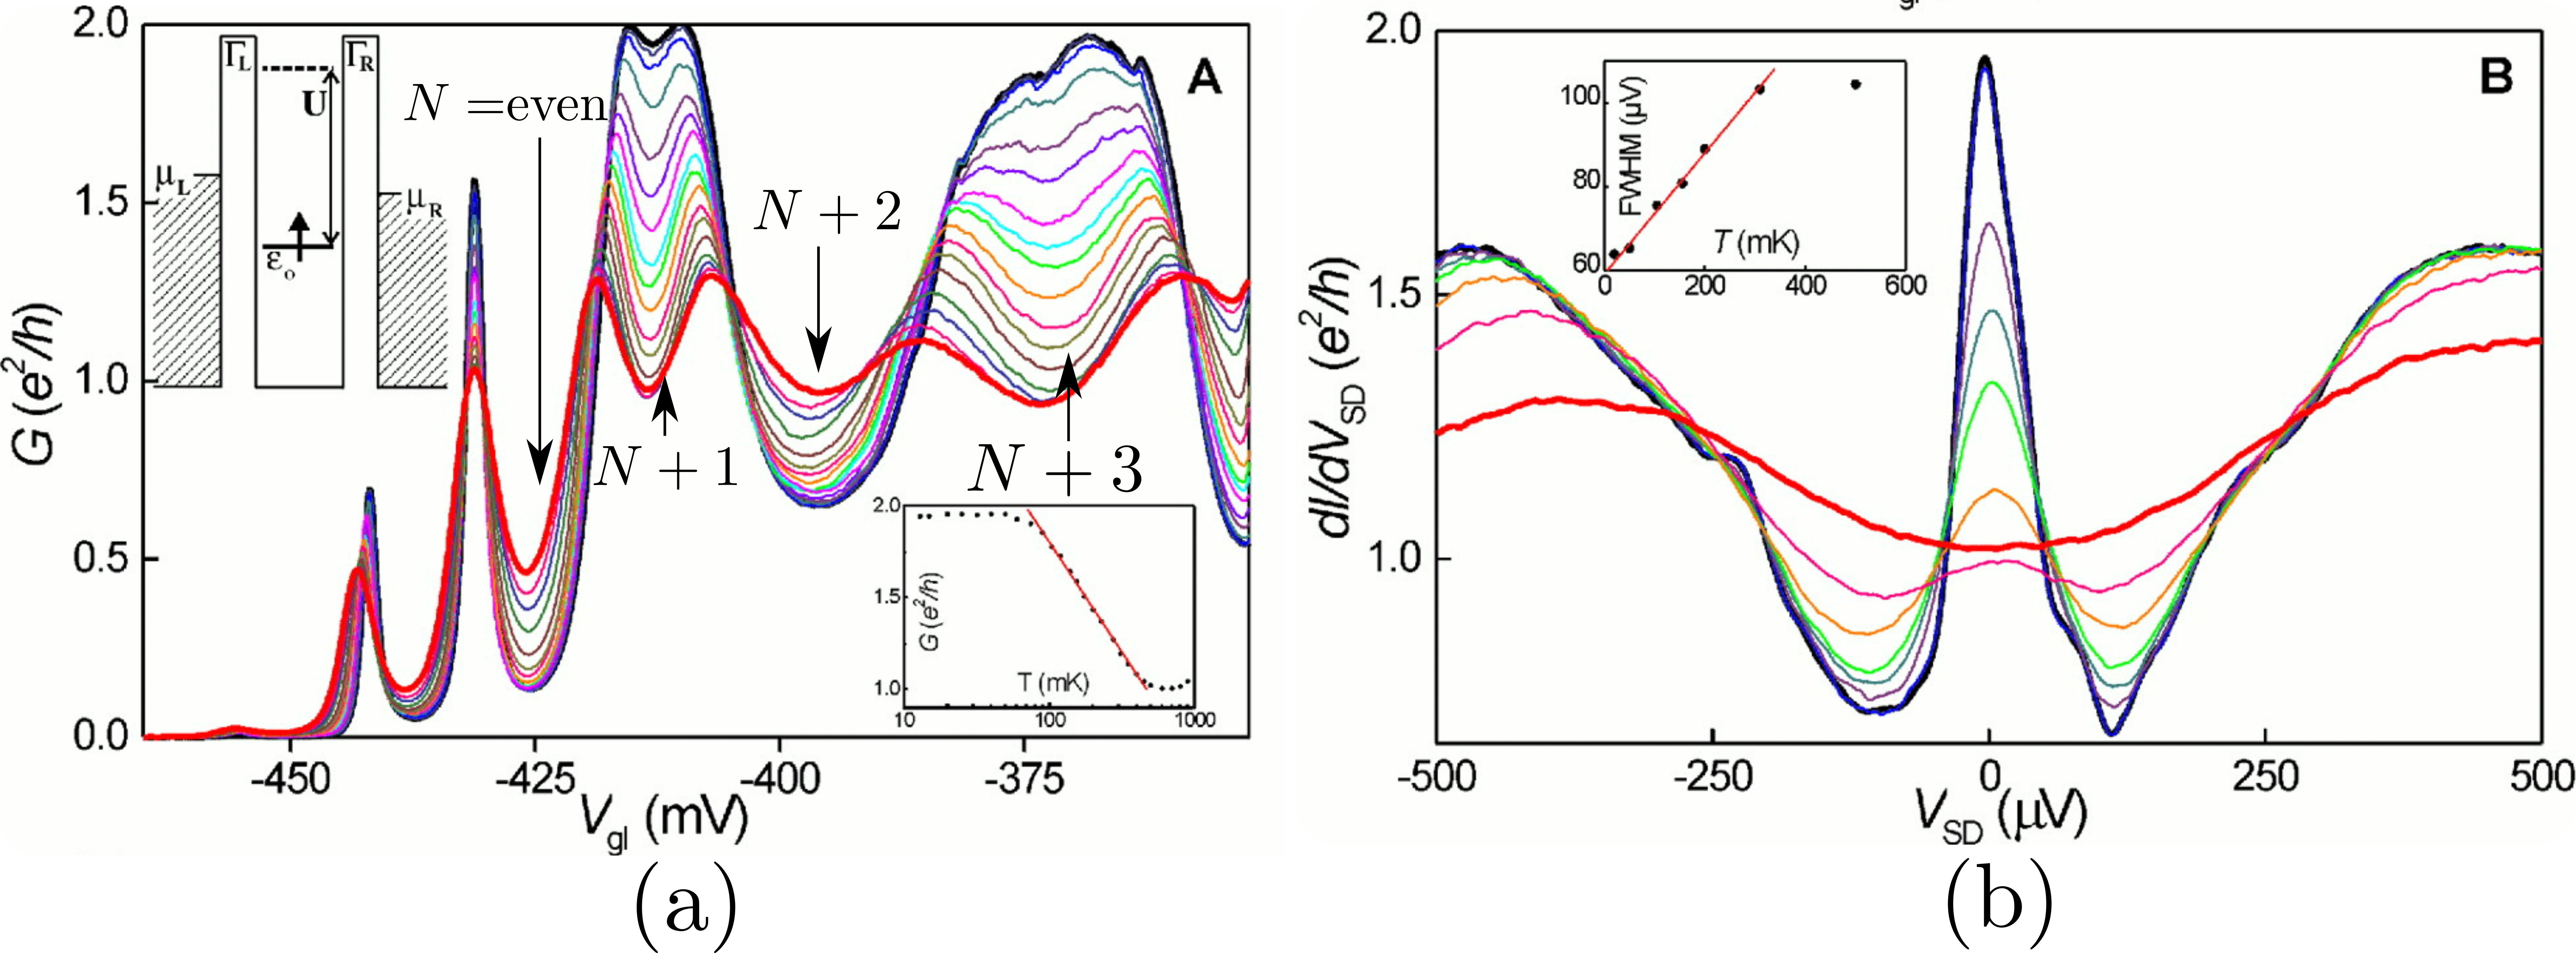
\includegraphics[scale= 0.28]{IMAGES/Preliminars/expKondoQD.png}
  \caption{ \label{fig:ExpKondo} Observation of the Kondo effect in a single electron transistor. Color scale temperatures from 15mk (Black) to 800mk(Red) a) Dependence of the zero bias conductance over the gate voltage. A plateau in the conductance peak appears in the odd particle regimes. b) Dependence of the conductance over the gate source drain voltage inside an odd electron regime. A zero bias conductance peak (ZBCP)  of height $\frac{2e^2}{\hbar}$ is observed. This is the Kondo signature.  \protect\Source{Adapted from \cite{wiel_kondo_2000}}}
\end{figure}


  The problem of magnetic impurities in metals can be treated using the Anderson model in a similar form as the transport in quantum dots. Hence, it is not a surprise that the Kondo Effect could also occur these systems. In 1998 the technological advances allowed the observation of the Kondo effect for the first time in a single electro transistor \cite{goldhaber-gordon_kondo_1998}. When an odd number of electrons is in the QD the last level bellow the Fermi energy is half-occupied, so that the dot can be considered as a magnetic impurity. The unlocalized electrons in the reservoirs then interact with this localized electron. Spin-exchange can occur as it happened with  magnetic impurities in metals. At low temperatures, this magnetic  interaction gives rise to strong quantum correlations that favor the formation of a singlet state between the localized electron and the electrons in the leads. As a result, the zero-bias density of states is increased producing a zero-bias conductance peak \ref{fig:ExpKondo}(b). 

Note that the physical implications of the Kondo effect  are different in magnetic impurities in metals and in QDs. In fact, they are complete opposite. While in magnetic impurities the resistivity increase, the Kondo effect in QD's leads no an unexpected raised in the zero-bias conductivity. The reason for this disagreement between both situations are the are the system dimensions. The scattering against a Kondo singlet in a  $3$D or $2$D systems against magnetic impurities is an obstacle to the conducting electrons. Instead, scattering in 1D-devices enhances the conductivity of the QD because there is only one scattering direction.

 As we previously discussed in \ref{sec:trans}, zero-bias transport in quantum dots can only occur if there is a state at the Fermi energy.  The Kondo effect creates a zero bias peak that is present whenever the dot has odd electrons . This explains the zero-bias plateaus observed in \ref{fig:ExpKondo}(a). We may think that the new singlet at the Fermi energy is creating a "channel" that allows quantum transport between both sides of the dot. This explains the Kondo peak. 

 In the following chapters we will give more details about this zero-energy-mode and theory that  explained it: The numerical renormalization group.  
















% The next part of thess preliminaries will be to compute the conductivity
% through the QD as a function of the gate voltage.
% In regular metals the Kondo effect manifests as a drop in conductivity
% under a certain Kondo temperature $(T_{Kondo})$ due to spin- scattering
% between the conduction electrons and the impurities of the material.
% The Anderson models, hence the NRG, are the perfect tools to study
% the physics of impurieties. Thus the computations we previously developed
% in this chapter will provide the right formalism to introduce the
% Kondo physics. This study will be an important part of the prelimiraries
% in the final document. 



%-----------------------------------------------------------


%\chapter{Motivation}
\section{Majorana Fermions}

The  Majorana Fermions, so called in the name of the Italian physicist Ettore Majorana, where first defined in the attempt to find a real solution of the Dirac equation. The real field that solves this equation $\Psi_M$ , describes a fermion which is its own antiparticle. Hence it has no electric charge nor mass.  Till these days, no fundamental particle with these characteristics has been observed. However, in the last few years, there has been a huge speculation about the possibility of finding Majorana Fermions as a quasiparticle inside certain condensed matter systems. 

One of the most famous examples of these systems is the Kitaev chain which is the main objective of the this subsection. 


\section{The Kitaev Chain}
The Kitaev chain is a toy model in tight binding that represents a  finite $p$-wave superconducting wire. The main Hamiltonian is given by 
\begin{equation}
H = \sum_{i} \left[ -t(a_i^{\dagger} a_{i+1} + a_{i+1}^{\dagger}a_i) -\mu a_i^{\dagger} a_{i} +  \Delta a_{i}a_{i+1} + \Delta^* a_{i+1}^{\dagger}a_i^{\dagger} \right].  \label{eq:kitaevHam}
\end{equation}

Where $\mu$ is the chemical potential, so that $\mu a_i^{\dagger} a_{i}$ is the energy associated to each free state. $t(a_i^{\dagger} a_{i+1} + a_{i+1}^{\dagger}a_i)$ represents the interaction between neighbouring sites which is determined by the hopping term $t$. The remaining terms describe the superconducting properties of the system as is is established by the BCS theory of superconductivity. $\Delta$ is a complex superconducting parameter with the form  $\Delta = e^{i\theta} \super$. The associated terms represent the Cooper pairs which can be created or annihilated at neighbouring sites of the system.

The form of hamiltonian \prettyref{eq:kitaevHam} favors the possibility of introducing new operators $\gammaA{j}$ and $\gammaB{j}$ such that

\begin{equation}
\gammaA{j} = e^{i\theta /2}a_j+ e^{-i\theta/2 } \ann_j \ \ , \ \ \gammaB{j} = -i(e^{i\theta /2}a_j - e^{-i\theta/2} \ann_j).
\label{eq:majoranaTrans}
\end{equation}
It is simple check that these operators are self-adjoint $(\gammaA{j}^\dagger = \gammaA{j}, \gammaA{j}^\dagger = \gammaB{j})$. This is a required constraint for the Majorana particles. In addition they satisfy the fermionic anti-commutation relations
\begin{equation}
\begin{aligned}
\{\gammaA{i}, \gammaA{j}\} = \{ & \gammaB{i} , \gammaB{j}\} = 2\delta_{ij}  ,\\ 
  \{\gammaA{i}, \gammaB{j} & \} =0.
\end{aligned} 
\label{majoranaRel}
\end{equation} 
This allows us to understand the operators $\gammaA{i} , \gammaB{i}$ as majorana fermions. If we also take the inverse of \prettyref{eq:majoranaTrans} we obtain that each  (Dirac) fermion in Hamiltonian \eqref{eq:kitaevHam} is composed by two majorana fermions such that 
$$a_j = \frac{e^{-i\theta/2}}{2}(\gammaA{j}+ i\gammaB{j})$$
We could even adventure to say that these majorana operators are actually dividing the Dirac fermions into real($\gammaA{}$) and imaginary $(\gammaB{})$ part ,the same way as complex numbers are a composite of two real numbers. 

The new Kitaev Hamiltonian in the Majorana representation looks like 

\begin{equation}
H = \frac{i}{2} \sum_{j} \left[ -\mu \gammaA{j}\gammaB{j}  + (t- \super) \gammaB{j}\gammaA{j+1} + (t+ \super) \gammaA{j}\gammaB{j+1} \right]+Const,\label{eq:HamMajorana}
\end{equation}

Depending on the values of parameters $\mu, t$ and $\super$ we can identify two regimes represented by the following situations:


%\begin{figure}[t]
%$$\includegraphics[scale=0.5]{KitaevtopPhases.jpg}
%\centering
%\label{top.phases kitaev}
%\caption{{\small \textit{Taken from \cite{bernevig2015topological}. Ilustration of the Kitaev chain for open boundary conditions in the Majorana representation. a)Represents the trivial case where the hopping and the superconducting term approaches to $0$. b) The non-trivial topological phase. The coupling is produced between Majoranas in different Dirac fermions }}}
%\end{figure}


\begin{enumerate}
\item{If $\super = t = 0, \mu <0$} Hamiltonian \eqref{eq:HamMajorana} becomes $\frac{-i\mu}{2} \sum_{j} \gammaA{j}\gammaB{j}$ which represents the coupling of the Majoranas in the same Dirac fermion. (See figure \ref{top.phases kitaev} (a))

\item{If $\super = t > 0, \mu =0$} the situation is much more interesting. The Hamiltonian \eqref{HamMajorana} takes the form $H = 2ti\sum_{j} \gammaA{j}\gammaB{j+1}$. This implies that the coupling is performed between  Majoranas of different Dirac fermions leaving the edge Majorana operators ($\gammaA{1}$ and $\gammaA{2}$) uncoupled . This produces a new degeneracy in the ground state due to the emergence of a state produced by the uncoupled Majorana operators. The new state is localized at the edges of the chain.(See figure \ref{top.phases kitaev} (b)) 
\end{enumerate}

%\chapter{Double QD coupled to a Majorana Bound State}

\begin{figure}[bh]
\includegraphics[scale=0.4]{IMAGES/2Dot-chain.eps}\caption{\label{Fig_2QD-Majorana} Two Qds ($a$ \& $b$) coupled to a TS sustaining
a Majorana Bound State(MBS) at the edge. To the other side they are
coupled to a methallic reservoir where conductivity is measured. }


\end{figure}


We now intend to study the transport properties through two QDs that
are coupled to a topological superconducting (TS) chain sustaining
a Majorana Bound State (MBS) as it is observe in \ref{Fig_2QD-Majorana}.
In \prettyref{sec:The-Numerical-Renormaliztion} we saw how the NRG
code can be applied to study the physics of transport through a QD.
In our case, we can set-up a similar Anderson-model to the one used
in \ref{eq:hamB0} taking

\[
H=H_{TS-2QDs}+H_{lead}+H_{int}=H_{M-QDs}+\sum_{\mathbf{k}\sigma l}\epsilon_{\mathbf{k}l}c_{\mathbf{k}\sigma l}^{\dagger}c_{\mathbf{k}\sigma l}+\sum_{il\sigma}V_{il}c_{\mathbf{k}\sigma l}^{\dagger}d_{i\sigma}+V_{il}^{*}d_{i\sigma}^{\dagger}c_{\mathbf{k}\sigma l}.
\]


with the new index $i\in\{1,2\}$ summing over both dots and $H_{TS-2QDs}$
representing the initial Hamiltonian system, which couples the two
Qds $\left(d_{1\sigma}^{\dagger},d_{2\sigma}^{\dagger}\right)$ with
the superconducting wire. The hamiltonian $H_{TS-2QDs}$ can be be
divided in three components

\[
H_{TS-2QDs}=H_{2QDs}+H_{int}+H_{TS}=H_{d_{i}}+\sum_{\sigma}\left(td_{1\sigma}^{\dagger}d_{2\sigma}+t^{*}d_{1\sigma}^{\dagger}d_{2\sigma}\right)+H_{int}+H_{TS}
\]


where $H_{d_{i}}$is the QD hamiltonian for dot $i$ \prettyref{eq:DotHam}
,$t$ is the hopping term between both dots, $H_{int}$is the dot-TS
interaction and $H_{TS}$ is the TS-hamiltonian . In \citep{vernek_subtle_2014},
the TS is modeled as a Kitaev chain \citep{kitaev_unpaired_2001}
and $H_{int}$ is the hopping interaction between dots and chain 

\begin{eqnarray}
H_{TS} & = & -\sum_{j=1}^{N}\mu a_{j}^{\dagger}a_{j}+\sum_{j=1}^{N-1}\left[-t'(a_{j}^{\dagger}a_{i+1}+a_{j+1}^{\dagger}a_{j})+\Delta a_{j}a_{j+1}+\Delta^{*}a_{j+1}^{\dagger}a_{j}^{\dagger}\right]\nonumber \\
H_{int} & = & \sum t_{i}d_{i\downarrow}^{\dagger}a_{1}+t_{i}^{*}a_{1}^{\dagger}d_{i\downarrow},\label{eq:Kitaev-dot}
\end{eqnarray}


where $a_{j}^{\dagger}$is the creation operator at site $j$ of the
chain, $t'$ is the hopping term between consecutive sites, $\Delta$
is the superconducting gap and $t_{i}$ is the hopping interaction
between the dot $i$ and the first site of the chain. We also assume
the dot only interact with spin-down $\downarrow$ operators in the
chain. \\

Using a Green's function approach on \prettyref{eq:Kitaev-dot} ,
\citet{vernek_subtle_2014} concludes that the Majorana mode at the
end of the chain leaks inside the QD when the TS is in the topological
phase . This fact favors a more simple effective model that has been
used in literature for simulation QD-TS interactions \citep{liu_detecting_2011,golub_kondo_2011,lee_kondo_2013}.
The model consists in considering only the coupling between the dots
and the Majorana modes that emerge in the topological phase. The resulting
hamiltonian is 

\begin{eqnarray}
H_{TS} & = & 2\epsilon_{m}\gamma_{1}\gamma_{2}\nonumber \\
H_{int} & = & \sum_{i}t_{i1}\left(d_{i\downarrow}^{\dagger}\gamma_{1}+\gamma_{1}d_{i\downarrow}\right)+it_{i2}\left(d_{i\downarrow}^{\dagger}\gamma_{2}+\gamma_{2}d_{i\downarrow}\right),\label{eq:Majorana-ham}
\end{eqnarray}


where $\gamma_{1,2}$are the two majorana operators and$t_{i1,2}$
are the hopping terms between the majoranas and the QDs.

The fidelity of this new model has been discussed by \citet{ruiz-tijerina_interaction_2015}
concluding that the majorana effective hamiltonian reproduces the
same results than the Kitaev chain model in the topological phase
(This statement is true even for more realistic models of the TS that
include Rashba spin-orbit interactions and a Zeeman field \citep{ruiz-tijerina_interaction_2015}
).\\

We now want to come back to a fermionic model, which was broken with
the introduction of majorana operators in the hamiltonian \prettyref{eq:Majorana-ham}.
For this we just need to replace the majorana operators $\gamma_{i}$
with their corresponding fermion operator

\[
f_{\downarrow}^{\dagger}=\frac{1}{\sqrt{2}}\left(\gamma_{1}-i\gamma_{2}\right)\ ,\ f_{\downarrow}=\frac{1}{\sqrt{2}}\left(\gamma_{1}+i\gamma_{2}\right)
\]


so that 

\[
\gamma_{1}=\frac{1}{\sqrt{2}}\left(f_{\downarrow}^{\dagger}+f_{\downarrow}\right)\ ,\gamma_{2}=\frac{1}{i\sqrt{2}}\left(f_{\downarrow}^{\dagger}-f_{\downarrow}\right).
\]


Supposing $t_{i1}=\left|t_{i1}\right|$ and $t_{i2}=\left|t_{i2}\right|e^{i\phi_{i}}$
to have a $\phi_{i}$-phase with respect to $t_{i1}$, we get to the
following hamiltonian 

\begin{eqnarray*}
H_{TS} & = & 2\epsilon_{m}f_{\downarrow}^{\dagger}f_{\downarrow}-\epsilon_{m}\\
H_{int} & = & \sum_{i}\tilde{t_{i-}}d_{i\downarrow}^{\dagger}f_{\downarrow}+\tilde{t_{i-}}^{*}f_{\downarrow}^{\dagger}d_{i\downarrow}+\tilde{t_{i+}}d_{i\downarrow}^{\dagger}f_{\downarrow}^{\dagger}+\tilde{t_{i+}}^{*}f_{\downarrow}d_{i\downarrow}
\end{eqnarray*}


with $\tilde{t}_{i\pm}=\frac{1}{\sqrt{2}}\left(\left|t_{i1}\right|-i\left|t_{i1}\right|e^{i\phi_{i}}\right).$
Therefore the final model for our initial hamiltonian is 

\begin{eqnarray}
H_{TS-2QDs} & = & H_{d_{i}}+\sum_{\sigma}\left(td_{1\sigma}^{\dagger}d_{2\sigma}+t^{*}d_{1\sigma}^{\dagger}d_{2\sigma}\right)\nonumber \\
 &  & \ \enskip\ \enskip+\sum_{i}\left[\tilde{t_{i-}}d_{i\downarrow}^{\dagger}f_{\downarrow}+\tilde{t_{i-}}^{*}f_{\downarrow}^{\dagger}d_{i\downarrow}+\tilde{t_{i+}}d_{i\downarrow}^{\dagger}f_{\downarrow}^{\dagger}+\tilde{t_{i+}}^{*}f_{\downarrow}d_{i\downarrow}\right]+2\epsilon_{m}f_{\downarrow}^{\dagger}f_{\downarrow}-\epsilon_{m}.\label{eqFinalMJ-2QDs}
\end{eqnarray}


The dimensionality of this system is $4\times4\times2=32.$ Again
we can write this hamiltonian by blocks using the preserved symmetries.
This time we can observe that the number of $\uparrow$-particles
$\left(N_{\uparrow}\right)$ is preserved in \ref{eqFinalMJ-2QDs},
but it is not for $\downarrow$-particles due to the terms $\left(d_{i\downarrow}^{\dagger}f_{\downarrow}^{\dagger},\ f_{\downarrow}d_{i\downarrow}\right)$.
However, the parity of $\downarrow$-particle $\left(P_{\downarrow}\right)$
is always preserved since $\left(d_{i\downarrow}^{\dagger}f_{\downarrow}^{\dagger},\ f_{\downarrow}d_{i\downarrow}\right)$
create or annihilate $2$-particles in the system. 

The final computations for $H_{TS-2QDs}$ in terms of the $N_{\uparrow},P_{\downarrow}$-symmetry
can be found in \prettyref{chap:Double-Dot-Majorana-Hamiltonian.}.
Setting $H_{-1}=H_{TS-2QDs}$ we can use the NRG algorithm \prettyref{eq:NRG-Iteration Hamiltonians}
to iteratively diagonalize this hamiltonian by 

\[
H_{N+1}=\Lambda^{\frac{1}{2}}\left[H_{N}+\frac{1}{2}\left(1+\Lambda^{-1}\right)\xi_{N}\left(f_{N\sigma}^{\dagger}f_{N+1,\sigma}+f_{N+1\sigma}^{\dagger}f_{N\sigma}\right)\right]\ \mbox{for \ensuremath{N\geq0}}.
\]


At $N=-1$ the equation above won't work since there are two QDs coupled
with the leads. The answer to this problem is simply to define constants
$\xi_{0i}$ that characterizes the coupling between dot $i$ and the
first opperator $f_{0}^{\dagger}.$ Thus we obtain 

\[
H_{0}=\Lambda^{\frac{1}{2}}\left[H_{-1}+\frac{1}{2}\left(1+\Lambda^{-1}\right)\sum_{i}\xi_{i0}\left(i_{i\sigma}^{\dagger}f_{0,\sigma}+f_{0\sigma}^{\dagger}d_{i\sigma}\right)\right]\ \mbox{for \ensuremath{N\geq0}}.
\]


This idea completes the NRG algorithm for the $2$QD-TS model coupled
to metallic lead. An NRG extension of the code developed by my thesis
advisor has been implemented \footnote{The code can be found in \url{https://github.com/cifu9502/nrgcode}}
and it is now in the error-correction stage. We hope for a rapid correction
of these errors to start running the program. 

%include{NResults}







\bibliographystyle{unsrtnat}
\addcontentsline{toc}{section}{\textbf{References}}
\bibliography{master,Majorana-QD,Kitaev-Majorana,Kondo}
\appendix
%dummy comment inserted by tex2lyx to ensure that this paragraph is not empty
\include{Abstract_A}
\include{AbstractB}
% Indices come here.

\end{document}
